%\chapter{Machine Learning for Metagenomics and Metatranscriptomics}
%\label{chapter:C}

\section{Abstract}

The potential to apply statistical/machine learning for metatranscriptomics data is explored, using the data of Chapter \ref{chapter:B}.
These data ($N$  = 88 samples, $d$ = 0.9 million measurements per sample) are too large to capture more than simple trends via manual inspections as is done in Chapter \ref{chapter:B}.
While typical machine learning datasets have much larger sample sizes ($N$), select regularized statistical learning techniques are promising.
This chapter focuses on two of them: canonical correlation analysis (CCA), and exploration of the approximated gene-expression partial correlation (pcor) matrix.
Results generated from this chapter are intended to generate hypotheses that will be tested with wet-lab experiments.
This chapter is left at an exploratory level; subsequent students will pursue the identified methods.


% ===========================
% ===== INTRODUCTION ========
% ===========================
\section{Introduction}

\subsection{Machine Learning for Metatranscriptomics}

\subsubsection{Essential Vocabulary}

Before jumping in, this subsection describes key vocabulary for statistical/machine learning.
"Sample" is used equivalently to biology, and the variable $N$ is used to denote the sample size.
In this experiment, $N$=88 for the 88 bottles that were sequenced.
"Feature" describes a measured value that is supplied to an algorithm.
A feature could be a raw measurement value (e.g. expression of gene A), or potentially some abstracted version of one or more measurements (e.g. $log$(expression), or (expression of A)*(expression of B).
The variable $d$ describes the number of features for each sample.

Machine learning is often used to make predictions, so there are terms to describe the different datasets used to train, validate, and test the models.
Ideally a new dataset is split into training data, and test data.
Training data are usually further split into chunks which can be iterated over to tune model "hyperparameters", a process called "cross-validation".
One example of a hyperparameter is the "regularization" strength, a measure of the penalty on large coefficients in models. % (discussed in Section XX).
These techniques allow tuning and evaluation of the model without compromising future predictive accuracy.

\subsubsection{Considerations for Meta-omics Data}

%Intro
The learning techniques chosen for this chapter were highly influenced by the properties of the underlying data.
These properties include sample independence, the samples size, compositional dependency, noise, high-dimensionality, and sparsity.
Each is described to contextualize model selection and analysis, and to aid in future consideration of other statistical frameworks.

\subsubsection{Non i.i.d. Sampling}
Machine learning techniques are generally applied to large datasets, where each data point is assumed to be independent and sampled from an identical data-generating processes (i.i.d.).
For example, a die that is more likely to roll a 6 if a 6 was just rolled exemplifies a violation of i.i.d.
Another violation example is a die that is more likely to roll a 6 when it is warm in the room.
The time-series nature and differences in \ce{O2} are analogous violations of i.i.d. assumptions for this dataset.
This i.i.d. violation can be beneficial, if perturbations allow more signal in the measurements, but can compromise generalizability.
Specifically, i.i.d. violations are more likely to produce models that are over-fit to the particular sample set and less likely to generalize to new data.
The concern about i.i.d. violations is set aside for this chapter given that wet-lab experiments will be designed to verify promising results.

\subsubsection{Sample size}
Machine learning is typically applied to datasets with sample sizes in the thousands or millions.
Some classic example domains include prediction of housing prices, or recognition of hand-written digits \cite{friedman2001}.
Access to tens of thousands of sample points allows the underlying structure to be discovered despite noisy measurements.
The data in this study have small $N$, limiting the number of frameworks that are appropriate.
In particular, this small $N$ is not suitable for generating predictive models.

In machine learning, predictive accuracy is tested by applying a model to un-seen data, and assessing the quality of the predictions.
Thus, one must have enough data to set aside test data that is never touched until the model is to be published.
The importance of not touching these test data until the model is published can not be over stated.
Assessing model accuracy on the test set before model development is complete often leads to over-fitting to the training data because the researcher will make subsequent modeling choices with those fit statistics in mind.
Given an $N$ of only 88, predictive models cannot be produced.
This is again consistent with the intention of this chapter to only use results for hypothesis generation.

\subsubsection{Compositional}
A further challenge of this dataset is that metagenomics and metatranscriptomics data are fundamentally compositional in nature: counts are sampled from a pool and absolute measures are not available \cite{tsilimigras2016, aitchison1982}.
As an illustration of the concern about compositional data, consider a hypothetical sample having only two genes: A and B.
Let genes A and B each have 1 unit of expression in a sample.
Then sampling of 60 reads leads (on average) to 30 reads counted per gene.
Now consider a second sample where B's expression is doubled but that of A remains constant.  When 60 reads are sampled again, only 20 will be associated with A and 40 will now be associated with B.
It thus appears that A's expression level has decreased when in fact only B's expression increased.
In the two-gene example above, the compositional effect is severe, however, as the number of expressed genes increases, the compositional effect grows less strong.

When multiple organisms are present, equivalent compositional effects occur across species.
Fluctuations in the abundance of one dominant organism can produce significant correlations for genes belonging to other microbial pairs that would be absent if comparing absolute measures of gene expression levels.
As with the example above, these cross-species compositional effects diminish as the number of abundant organisms increases.
In the limit of large community complexity, the compositional nature of metatranscriptomics/metagenomics data can be neglected \cite{tsilimigras2016}.
This thesis assumes that the diversity of abundant organisms and number of expressed genes is high enough to find real biological signal above the effects of compositional artifacts.

\subsubsection{Noise}
Consideration of experimental noise is necessary for analysis of metagenomics/metatranscriptomics data, as there are many noise-generating steps.
The first source of noise is biological variation.
Different samples have different population evolution trajectories.
These are often driven by unknown latent variables, and thus cannot be controlled for.
There is also noise that is common to all sequencing datasets, such as amplification biases, sequencing biases, etc..

Additional layers of noise are added when inferring the origin of these reads.
The reference DNA to which reads are mapped is known to be imperfect (see Figures \ref{fig:4dominant_groups}, \ref{fig:rna_mapping_bars}), so the tabulated RNA-seq measurements carry uncertainty.
On top of that, there is ambiguity in how to count reads that map equally well to two or more places \ref{sect:multipli_mapped_reads}).
This chapter explores the potential of finding signal in spite of these unavoidable layers of noise.

\subsubsection{High Dimensionality}
%Example of over-fitting
High dimensionality relative to the sample size can lead to over-fit models if model complexity is not limited \cite{friedman2001}. % pg 38: bias variance trade-off.
For example, consider a housing price dataset with $N$=100 houses, and $d$=1,000 measurements including some presumably uninformative measurements such as the number of steps to the front door, and the last digit of street address.
If only ten variables are allowed in the model, fitting is likely to select the most influential variables (e.g. square footage).
However, if an arbitrarily large model is allowed, the model is likely to include the nonsense features.
Thus it is essential to limit model complexity when $d$ is larger than N.
Regularization is a common technique that adds an additional term to the objective function which penalizes large coefficients \cite{friedman2001}.
Regularization strategies are discussed below, and featured in all techniques highlighted in this chapter.

\subsubsection{Sparsity \& Heavy-tails}
%Sparsity
Many of the metatranscriptomics read count measurements for the 0.9 million genes are zero, indicating high sparsity.
For the 754,836 genes found to have nonzero expression in at least one sample, only 10.6\% of read count values are nonzero.
    % 0.10595531527859875.  See np.count_nonzero(read_counts, axis=1)/elements*1.0 in /misc 170403_iid_and_non-gaussian_figures
To illustrate, Figure \ref{fig:sparse_RNA-seq} shows the read counts for 150 randomly selected genes (columns) across samples(rows).
White rectangles indicate zeros.  All nonzero values are highlighted in color.
Many algorithms are not designed to handle this level of sparsity.
For example, models that use Gaussian (normal) distributions to represent the underlying data should not be assumed to handle sparsity, unless explicitly stated.

%Heavy-tailed distributions
The distributions of counts are also heavy-tailed: large read counts are less common than small counts.
Sparsity aside, these tails are problematic for many model classes, including those based on Gaussian distributions.
%The majority of methods explored in this chapter transform the raw distribution, or statistics derived from them.
The models selected in this chapter are reasonable choices given the sparsity and heavy tails, though even stronger adaptations of these models for high sparsity are likely available in the statistics literature if subsequent students are open to programming their own algorithms.


%\subsection{Canonical Correlation Analysis of Metagenomic Gene Expression}

\begin{figure}[H]
\centering
    % Original: /Users/janet/Documents/Lidstrom Lab Work/meta4_bins_data_and_files/170403_sparsity_and_heavy_tails/20170403_sparsity_illustration--754836_nonzero_features.pdf
    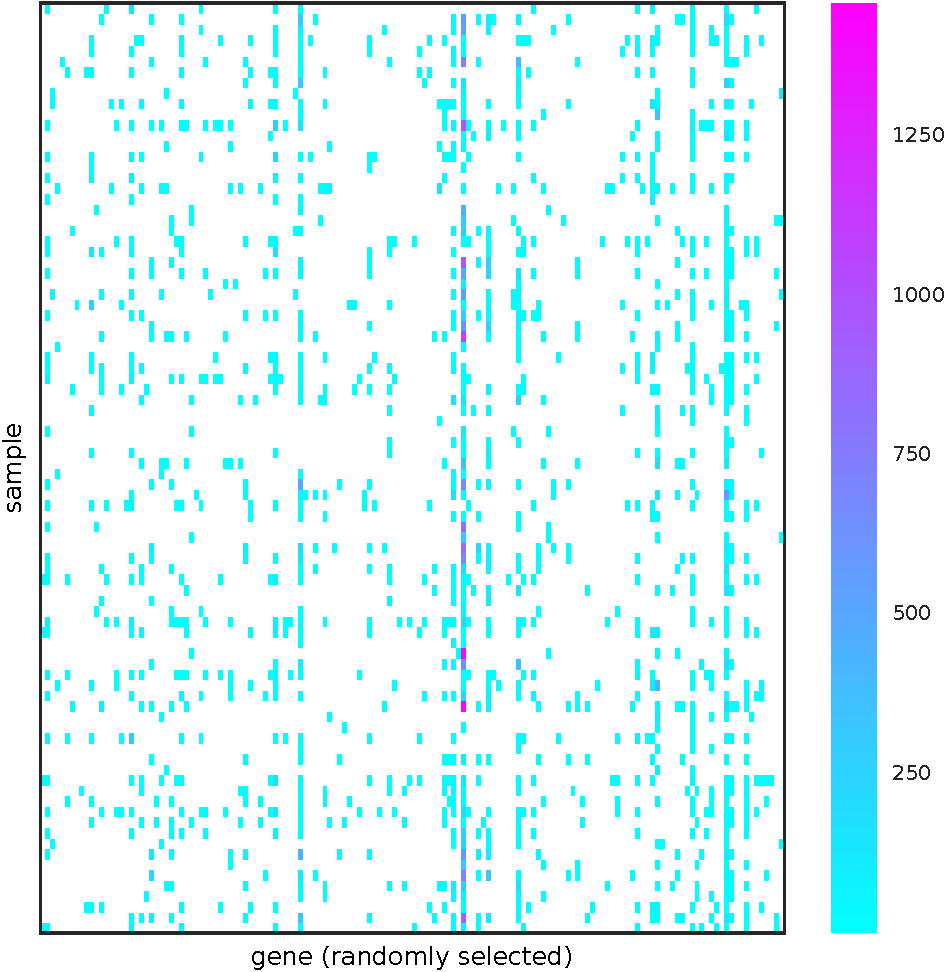
\includegraphics[width=0.8\textwidth]{./tex/chapter3/figures/20170403_sparsity_illustration--754836_nonzero_features.pdf}
    \begin{singlespace}
    \caption[Illustration of the sparsity of the RNA-seq count data]{
        Illustration of the sparsity of the RNA-seq count data.
        Nearly 90\% of measurements of reads per gene per sample are zero, even after removing genes zero reads mapped across samples.
        }
    \label{fig:sparse_RNA-seq}
    \end{singlespace}
\end{figure}


\subsection{General Steps}

%Though preparations for machine learning vary significantly
There are many types of machine learning approaches in the literature.
There are, however, three nearly universal steps for common to all: data normalization/standardization, choice of strategy to limit model complexity, and cross validation.
Each is described below.

\subsubsection{Standardization}
First, standardization of the data is almost always done.
Poor fits are often obtained when features/measurements are on different scales (e.g. inches and miles).
Even if measurements are in comparable units, many algorithms perform better when the features are scaled such that the variances are on a similar scale.
This chapter always scaled the features so each gene had variance = 1, but found centering of features (shift so the mean = 0) to be harmful (see Section \ref{sect:centering_sparse}).

\subsubsection{Model Class Selection \& Limiting Model Complexity}
Next, an appropriate model class needs to be selected.
As discussed above, consideration of $N$ and $d$ have large influence on model selection.
With $N$ = 88 and $d$ = 0.7 million, extra care to limit model complexity is essential.
Fancy algorithms with many parameters (e.g. neural networks) are inappropriate; models that can be limited to a small number of parameters were sought instead.
The two most common penalties for limiting model complexity are L1 (a.k.a. "lasso") \cite{tibshirani1996} (absolute values of coefficients are penalized) and L2 \cite{hoerl1970} (squared coefficients are penalized).
Both limit the coefficient sizes, but L1 leads to more truly zero coefficients \cite{tibshirani1996} and is thus particularly appealing in the $d >> N$ regime, or when some features are expected to be uninformative.
L1 penalties are used by algorithms in several of the methods explored herein.

\subsubsection{Cross Validation} %Evaluate fairly
As emphasized previously, the greatest danger of machine learning is production of a model that will not generalize to future un-seen data.
This can occur because of poorly selected model hyperparameters.
The best practice approach for choosing hyperparameters is cross-validation, whereby the models are trained multiple times, each time with a different portion of the data set aside as a validation set.
The held-out validation set is used to assess the performance of the model trained on the the remaining fraction of the data.
Such cross-validation provides the best framework for tuning parameters without touching the test data, thus reducing over-fitting.

\section{Methods explored}
Machine Learning encompasses broad sets of tools that can be as simple as linear regression or as potentially complex as neural networks.
This chapter uses canonical correlation analysis, a classical statistical tool, and various methods of obtaining and exploring graphs based on the gene-expression partial correlation matrix.

\subsection{CCA}
%Intro
Canonical correlation analysis (CCA) is a classic method dating back to 1936 \cite{hotelling1936} that highlights relationships between two sets of variables \cite{sherry2005}.
In particular, CCA identifies linear combinations of variables that maximize the correlations \footnote{Pearson r, thus "Canonical Correlation" \cite{sherry2005}} between measurements in two matrices.
It can be used as a statistical learning algorithm when the vectors produced predict gene expression of new data that have not been used to fit or assess the model.
In this chapter, if reasonable prediction at the cross-validation step is seen, the genes included in those vectors could highlight interesting biology to target with subsequent experiments.
The utility of CCA was explored by testing for correlation between a linear combination of a set of methylotroph genes and a linear combination of a set of methanotroph genes.
The data used were the tabulated RNA-seq reads after alignment to the 55 isolate genomes, allowing for labeling of species category.
% TODO: Cartoon of vectors.
% TODO (?) Similar to PCA.  PCA explains variance, CCA explains correlation

%Sparsity
The large number of features ($d$) relative to the number of samples ($N$) motivated use of a variation that produces sparse vectors.
In other words, a method was sought that could use regularization to pick out a handful of genes (features) in each category, rather than all features.
The R package PMA\footnote{\url{https://cran.r-project.org/web/packages/PMA/PMA.pdf}} \cite{witten2009} was selected.
CCA variants that focused on both sparsity and compositional data were not found.

\subsection{Gene Expression Partial Correlations}

%Intro
The observational studies of Chapter \ref{chapter:B} were not able to answer the pressing question of what drives the changes in community composition and the patterns of organism distribution (see Figures \ref{fig:4dominant_groups}, \ref{fig:dominant_genera}).
What drives the higher abundance of methylotrophs in the high \ce{O2} samples?
What makes some samples more likely to have high abundances of Bacteroidetes or Burkholderiales?
Do certain methylotrophs flourish when certain methanotrophs express particular sets of genes?

The trends of which genes tend to be co-expressed across samples can help answer these questions.
Correlations are not the best measure to infer causality, as they detect independence rather than dependence \cite{schafer2005}.
%Correlation between gene expression levels can hint at causality, but of course correlation does not imply causality.
A better measure is partial correlation, which measures the strength and directionality of a linear relationship between two variables while controlling for the effects of other variables.
Partial correlations are more likely to be linked to causality than correlations, but are also more difficult to estimate when $d > N$ (see below). % (see Section XX) .

The set of partial correlations can be represented as a graph describing how species interact.
Genes can be represented by nodes, and edges can be added for genes with significant partial correlations \cite{borthagaray2014}.
Once a graph is in hand, community structure can be detected by searching for groups of nodes that are highly connected to each other but have fewer connections to nodes outside the group \cite{hero2012}.
Edges that are labeled by organism type and/or taxonomy can be used to find sub-structures including multiple species.

A reduced version of the partial correlation matrix is desired.
For a network of 0.7M genes (7.0E5), there are approximately 0$.7M^2/2$ ($0.7E11$) potential partial correlation values. % really d(d-1)/2
These partial correlations can be represented in a matrix, or equivalently as edges in a graph.
Clearly the majority of edges are not expected to have meaningful partial correlations, so the goal is to identify the handful of edges that that highlight meaningful biology.
Furthermore, in this $d >> N$ regime, the traditional partial correlation matrix is ill-formed \cite{whittaker2009} such that shrinkage \footnote{similar to regularization} is required.
%In addition, estimation of the partial correlation matrix with this high dimensionality leads to mathematical instability.

There are many potential algorithms that can estimate the reduced set of partial correlations and highlight interesting biology in $d >> N$ regimes.
The Strimmer lab has made great advances in this area \cite{schafer2001, schafer2005, opgen2007shrinkage}.
One Strimmer Lab method uses a shrinkage formula (see the R package \texttt{corpcor}\footnote{\url{http://strimmerlab.org/software/corpcor/index.html}}) and analytic approximations that leads to an estimation of the thinned partial correlation matrix from the gene counts matrix.
They use a shrinkage parameter that shrinks the empirical correlations towards the identity matrix, while leaving empirical variances intact.
While promising, their methods have not been applied to larger omics sets.
The Strimmer group's 2005 paper uses 4,289 genes of \textit{E. coli} and 8 RNA-seq samples \cite{schafer2005}.
The 2007 paper used 800 pre-selected \textit{Aradopsis thaliana} genes \cite{opgen2007Aradopsis}.
%  4,289 protein coding genes of E. coli 8, 15, 22, 45, 68, 90, 150, and 180 minutes after induction of the recombinant protein SOD http://strimmerlab.org/publications/journals/shrinkcov2005.pdf
%In fact, many of their demos are not even demonstrated on the whole set of a single organisms' genes (cite).
This chapter explores the potential of using their methods on larger and higher-sparsity metatranscriptomics data.

Ledoit-Wolf is another route to that uses an empirical rule (no need for cross-validation) to estimate the inverse correlation matrix \cite{ledoit2003}.
This inverse correlation matrix is proportional but not equal to partial correlations.
Further thinning of the network with something such as false discovery rate corrections can be used to thin edges \cite{opgen2007Aradopsis}.

Graphical lasso is another promising method of producing the desired partial correlation network \cite{friedman2008}.
This technique uses L1 regularization to directly compute a sparse matrix of partial correlations.
Cross-validation can be used to optimize the regularization strength.

\subsubsection{Mining the Partial Correlation Matrix}
Even a sparse partial correlation matrix requires computational tools to investigate.
If the top 5\% of potential partial correlation values are kept, this is still $0.05*(1.4E11) = 7.0E9$ edges.
The graphs can be explored by a variety of methods, including NetworkX\footnote{\url{https://networkx.github.io/}} (Python) \cite{schult2008}, and the specialized graph database Neo4j\footnote{\url{https://neo4j.com/}}.

\subsection{Taxonomy of Genes and Contigs}
Knowledge of the taxonomy of genes and contigs are necessary for finding interesting cross-species interactions.
For CCA, taxonomy labels allow separation by microbe type (e.g. methanotrophs vs methylotrophs).
Labels of species in gene-expression partial correlation graphs allow identification of cross-species edges and sub-graphs that include genes from multiple species.
These taxonomic labels can be done at contig level, or the gene level.
Ideally labels at both levels are consistent.

Several methods for obtaining taxonomic labels were explored.
Most tools that assign taxonomic labels (e.g. MEGAN \cite{huson2015}, Kaiju \cite{menzel2016}, Taxator-tk \cite{droge2014}, MetaPhlAn \cite{segata2012}) are designed for individual raw sequencing reads rather than contigs.
Caution must be used when extending these methods to contigs, due to the larger length of contigs and the variable sizes.
For example, taxonomy calls may be made on short, say 100bp regions, of 100kb contigs.
If that region is representative of the whole contig, than a short match works great.
However, aggregating information about matches along the length of the contig should be more robust.

There are few tools designed for contig taxonomy assignments available.
MyTaxa aims to classify contigs using an extension of the Average Amino Acid Identity (AAI) concept \cite{konstantinidis2005}.
This tool was also tested, but appears to be broken and shows no signs of recent maintenance.
Currently a tool for per-gene taxonomic classifications using BLAST best hits and large word sizes is being developed by David Beck.
Additional tools will be required to infer taxonomy across whole contigs, as the labels for genes within a contig will not always agree.


% ================================
% ===== MATERIALS/METHODS ========
% ================================
\section{Materials and Methods}

The data used are RNA-seq counts described in Chapter \ref{chapter:B}.

\subsection{Taxonomy Predictions}
Kaiju \cite{menzel2016} was tested for the ability to predict contig taxonomy.
The settings used included \texttt{-a greedy -e 10000 -x}: greedy mode with up to 10,00 mismatches and filtering of query sequences containing low-complexity regions.
As discussed below (Section \ref{results:taxonomy}), concern about predictions of the taxonomy of long contigs using small portions of their coding sequence led to exploration of BLAST-based methods.
MEGAN was downloaded but was not pursued due to poor support for the command line interface.

\subsection{Canonical Correlation Analysis (CCA)}
CCA was applied to the mappings of the metatranscriptomes of Chapter \ref{chapter:B} to the 55 isolate genomes, in units of RPKM.
Expression levels across genes with the same gene name were pooled.
These data were then split into two matrices: one contained all genes from methanotrophic species and the other contained genes from the non-methanotrophic methylotrophic species.
Gene products having zero variance were removed.

%Features appearing in less than XX of samples were removed.
Each feature was normalized by scaling the variance to 1 with Python's StandardScaler\footnote{\url{http://scikit-learn.org/stable/modules/generated/sklearn.preprocessing.StandardScaler.html}}, but was not centered to have zero mean due to sparsity concerns.
Cross-validation was done to assess predictive accuracy across regularization strengths.
Penalties for the two matrices were kept at the same value, rather than use of a grid search.  %?? Did I ever grid search?  Appears not
% vl = [0.1, 0.2, 0.3, 0.4, 0.5, 0.6, 0.7, 0.8, 0.9]
% [(v, v) for v in vl]
R code was called from Python through rpy2\footnote{\url{https://rpy2.readthedocs.io/en/version_2.8.x/index.html}} \cite{gautier2008}.
All code is available on GitHub: \href{https://github.com/JanetMatsen/CCA_Omics}{CCA\_Omics}.
% TODO: sum on gene product by name.   Reduce number of features.

\subsection{Estimating the Partial Correlation Matrix}

\subsubsection{Prepping Data: Trimming and Normalization}
Data was trimmed and normalized before partial correlation calculations were performed.
First, genes with zero reads assigned across all samples were removed, bringing down the number of features from ~0.9 million to ~0.75 million genes. % 921435 --> 754836
Next, variants of these data with different total numbers of features were prepared by varying a cutoff that accounted for sequencing depth.
The criteria for inclusion was contribution of a specified fraction of reads in at least one sample.
This measure allowed features that were important in one sample, regardless of sequencing depth, to be included.
Dividing by the fraction of reads mapped to coding sequences seemed reckless given low fractions of reads mapped to coding sequences (see Figure \ref{fig:rna_mapping_bars}).
These datasets of varying size were used to test how well various algorithms to scale to this large dataset.

Three approaches were used to approximate the partial correlation matrix: (1) Ledoit-Wolf estimation \cite{ledoit2003}, followed by removing small-magnitude edges, (2) Graphical Lasso \cite{friedman2008} with varying regularization strengths, and (3) the GeneNet \footnote{\url{http://strimmerlab.org/software/genenet/}} package \cite{schafer2001, schafer2005}.
For all three approaches, the variance of each feature was scaled to 1 prior to training the models.
All three were tested on large-memory (244 Gb) AWS instances.

\subsubsection{Ledoit-Wolf}
Estimates of the pseudo-inverse matrix, a matrix proportional to the partial correlation matrix, was estimated via the Python implementation of Ledoit-Wolf\footnote{\url{http://scikit-learn.org/stable/modules/generated/sklearn.covariance.LedoitWolf.html}}.
Data sets of increasing size (increasing number of genes) were tried on an EC2 \texttt{r4.8xlarge} (244GB memory) instance.
The fact that values produced are proportional but not equal to partial correlations prevented use of edge-thinning via false discovery rate tools such as fdrtool\footnote{\url{https://cran.r-project.org/web/packages/fdrtool/fdrtool.pdf}}, which only accept test statistics.
Instead, the partial correlations with the largest magnitude were extracted.
Specifically, the 2.5\% of edges with the most positive, and 2.5\% of the edges with the most negative values were retained.

\subsubsection{Graphical Lasso}
Graphical Lasso was also tested, again with increasing file sizes.
The Scikit-Learn implementation\footnote{\url{http://scikit-learn.org/stable/modules/generated/sklearn.covariance.GraphLasso.html}} \cite{scikit-learn} (Python) was tested, as well as the Huge\footnote{\url{https://cran.r-project.org/web/packages/huge/huge.pdf}} \cite{zhao2012}  package of R, which promises better scalability for large data.

\subsubsection{GeneNet Package}
GeneNet\footnote{\url{https://cran.r-project.org/web/packages/GeneNet/GeneNet.pdf}} was called from R.
This package uses an analytic shrinkage estimator of the correlation matrix, so cross-validation was not required.
%Ran in R (see \href{https://github.com/BeckResearchLab/meta4/blob/master/rnaseq/pcor_new/GeneNet/run_GeneNet_and_summarize.R}{R script}).
Again, genes were trimmed out of the input data if they contributed less than a specified percent in all 88 samples.
The top million edges were explored.

\subsection{Exploring Networks}
%Intro
Different tools were used to explore the resulting matrix structures, in graph form.
Regardless of the software used, the general graph structure included nodes as genes, and edges as partial correlations.
%Nodes were also labeled with taxonomy.

\subsubsection{NetworkX}
Tabular data with one row per edge were loaded into Pandas.
Unique loci were identified, then loaded into NetworkX.
Edges were added by iterating over edge dataframes.
NetworkX haas built-in methods for computing basic network properties such as average connectedness.
See Python code \url{https://github.com/BeckResearchLab/meta4/blob/master/rnaseq/pcor_new/networkx/networkx_helpers.py}.

\subsubsection{Neo4j}
Use of Neo4j was also explored (see \url{https://github.com/JanetMatsen/Neo4j_meta4}).
This database-specific program has a particularly powerful query language, but is slow to develop in without Java programming skills.
A Python API is available, but is more limited than the Java API.


% =================================
% ===== RESULTS/DISCUSSION ========
% =================================
\section{Results and Discussion}

\subsection{Taxonomy Predictions}
\label{results:taxonomy}
Taxonomy calls at the gene and contig level were sought to enable applications of statistical learning that probe interactions between microbes.
While Kaiju produced usable taxonomy calls for the majority of contigs, exploration of these data raised concerns about extrapolation of taxonomic assignments from small match regions to long contigs. %to small regions of the contig to the length of contigs up to XX kb.  %  XX percent of contigs
Currently David Beck is developing a tool for BLAST-based taxonomic assignments of individual genes.
These assignments will be rolled up into contig-level taxonomic predictions.
The statistical learning technique results described below could not use contig taxonomy predictions, but future directions that use this rich layer of information are proposed.

\subsection{Avoid Centering Sparse Data Prior to Learning}
\label{sect:centering_sparse}
Early work for this chapter highlighted the importance of not centering scaled features during preprocessing (Figure \ref{fig:standard_scaler}).
The sparsity of metagenomic data leads to peaks at zero being shifted away from zero during centering. % is not amenable to centering, or the zero peak can is shifted.
The heavier the tail, the greater the shift. %more this peak is shifted away from zero.
These shifted peaks led to strange artifacts in modeling, so centering during preprocessing was always avoided.

\begin{figure}[H]
\centering
    % Originals: /Users/janet/repos/CCA_Omics/code/demo_notebooks/results_for_thesis/170324_example_centered.svg
    % Merged: /Users/janet/Dropbox/thesis/inkscape/170324_standard_scalar.svg.2017_03_24_07_44_42.0.svg
    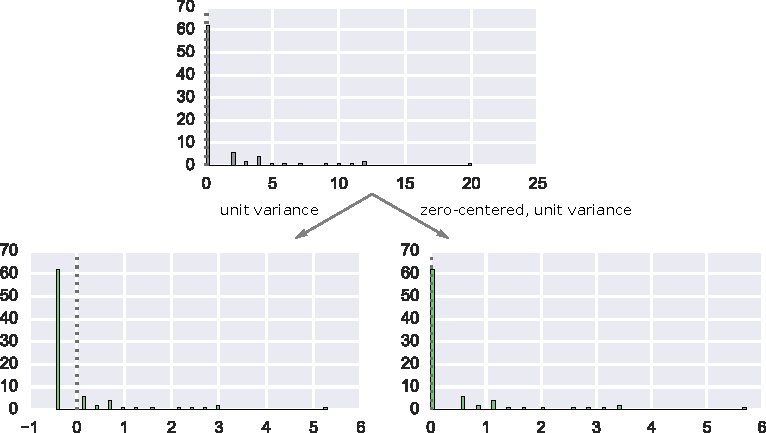
\includegraphics[width=0.8\textwidth]{./tex/chapter3/figures/170324_standard_scalar.pdf}
    \begin{singlespace}
    \caption[Feature scaling: centering sparse features is not advised]{
        When preparing features for machine learning, centering sparse data is not advised.
        All plots have read counts (RPKM, with or without scaling) on the x-axis and the number of samples on the y-axis.
        The top plot shows the untransformed distribution of RPKM for a particular copy of a gene encoding
            "methane monooxygenase component A alpha chain".
        The gene is not expressed in many of the samples, giving the large peak at zero.
        Below, two different normalization schemes are shown:
            standardization so the variance is 1 (left), and
            standardization so the mean is zero and the variance is 1 (right).
        Most machine learning algorithms will produce models with problem artifacts when fitting to such shifted-zero peaks.
        }
    \label{fig:standard_scaler}
    \end{singlespace}
\end{figure}

The CCA results were particularly problematic when features were centered.
Specifically, very high correlations were predicted, but only using features where most measurements had been zero prior to centering.
Variants of CCA that are designed to produce sparse results from sparse data were searched for, but not found.

\subsection{Partial Correlation Matrix Estimation}

\subsubsection{Graphical Lasso}
None of the methods for estimating the partial correlation matrix scaled well to the entire 0.75 million gene dataset.
% TODO: try GeneNet on the whole 0.7M feature data.
The general strategy for exploring algorithm scalability was to run each pipeline on input datasets of increasing size.
The Scikit-learn implementation of Graphical lasso scaled particularly poorly, struggling even with the top 815 features.
It produced floating point errors. % \texttt{FloatingPointError}s:
\texttt{FloatingPointError: Non SPD result: the system is too ill-conditioned for this solver.} % The system is too ill-conditioned for this solver}
In addition the necessity to tune the regularization strength via cross-validation added substantial compute requirements.
Further exploration of this tool is not suggested, unless a few dozen genes have been pre-selected for exploration, as was done in the Strimmer Lab papers.

%\subsubsection{Huge}
The Huge package's variant of graphical lasso scaled better to larger data than the Scikit-learn graphical lasso implementation, but still could not solve large networks.
Instead, other techniques were pursued.

\subsubsection{Ledoit-Wolf}
The Scikit-learn Ledoit-Wolf algorithm scaled reasonably: it was able to approximate the partial correlation matrix for the top 26,968 genes.
The values it reports, however are inverse covariance matrix values, not the partial correlation matrix.
The inverse covariance matrix values are proportional to the partial correlations, but they are not true partial correlations.

Furthermore, genes that are expected to have positive partial correlations in fact had negative values.
To verify this trend, a minimal example was prepared.
The values of 9 genes corresponding to three \textit{pmoCAB} clusters were used, and again the expected within-operon precision matrix values were negative (Figure \ref{fig:pcor_pmocab}).
This may be the result of an unexpected sign convention that is not described in the Python documentation.
Further reading of the Whittaker textbook \cite{whittaker2009} could elucidate the steps needed to get from inverse covariance estimates to partial correlations, and clarify this sign issue.

\begin{figure}[H]
\centering
    % /Users/janet/Dropbox/thesis/tex/chapter3/figures/170403_pMMO_pcor_heatmap.pdf
    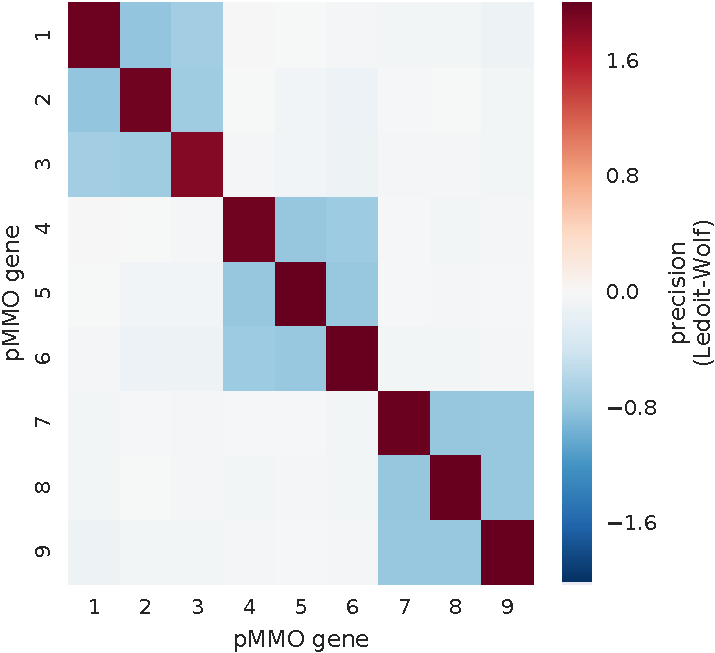
\includegraphics[width=0.7\textwidth]{./tex/chapter3/figures/17045_LedoitWolf_results_on_9_pmo_genes--uncentered.pdf}
    \begin{singlespace}
    \caption[Partial correlation demo: three \textit{pmoCAB} clusters]{
        %The matrix inverse of the covariance matrix, often called the precision matrix, is proportional to the partial correlation matrix
        Ledoit-Wolf estimated precision matrix values (proportional to partial correlations) for a minimal example of 9 genes in three different three-gene \textit{pmoCAB} clusters.
        The read counts were scaled to unit-variance prior to application of the Ledoit-Wolf function in Python's scikit-learn.
        %Notably, the partial correlations for all within-cluster pMMO subunits are negative.
        }
    \label{fig:pcor_pmocab}
    \end{singlespace}
\end{figure}


\subsubsection{GeneNet}
GeneNet provided excellent estimates of the partial correlation matrix.
The algorithms scaled well, despite previous publications having focused on tens or hundreds of genes.

Sequential genes in clusters proved to have the expected positive-valued partial correlations, and an input file of the top 26,968 genes produced partial correlation estimates in about 6 hours on an AWS \texttt{r4.8xlarge} instance (244GB memory). %31,767
Larger networks produced memory errors.
%Larger networks were not tried, as the lowest expressed features are less likely to produce interesting biological stories.

\subsubsection{Validation of the GeneNet Partial Correlation Graph}

Partial correlation graphs were explored with NetworkX and Neo4j.
NetworkX has the large advantage of being quick to program for Python developers, but Neo4j has a much more powerful query language.
The Neo4j query language allows such queries as
%\texttt{MATCH (n)<- [e \{cross_species:'True'\}] -> (m) WHERE n.gene\_product =~'.*transport.*' AND e.pcor\_abs > 0.045 RETURN n, m}
\begin{verbatim}
MATCH (n)<- [e {cross_species:'True'}] -> (m)
    WHERE n.gene_product =~ '.*transport.*'
        AND e.pcor_abs > 0.02
    RETURN n, m
\end{verbatim}
This query demonstrates restriction to cross-species edges where the first gene product of the first node contains the substring``transport" and the partial correlation magnitude is above 0.02.
Neo4j may be used more in future analysis, but the short-term goals of probing the basic network structure were better done using NetworkX.
% gene product of the

%Basics
The top 1 million partial correlation values (edges) had the following distribution (Figure \ref{fig:pcor_hist}):
\begin{figure}[H]
\centering
   % /Users/janet/Documents/Lidstrom Lab Work/meta4_bins_data_and_files/170412_explore_specific_network_as_done_previously/170412_explore_cutoff_0.01/pcor_hist--1e+06_edges.pdf
    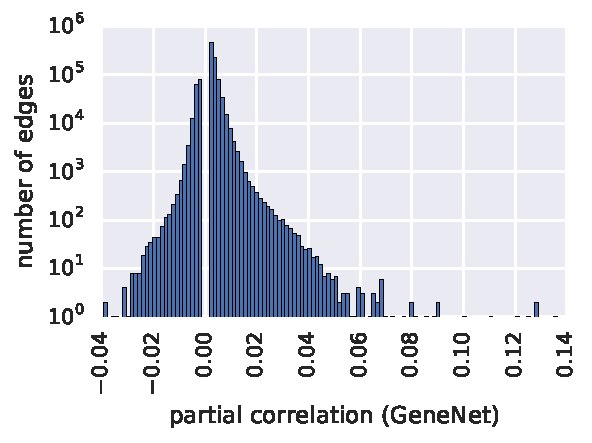
\includegraphics[width=0.6\textwidth]{./tex/chapter3/figures/pcor_hist--1e+06_edges.pdf}
    \begin{singlespace}
    \caption[Distribution of the 1 million partial correlation values with the largest magnitudes]{
        Distribution of the 1 million partial correlation values with the largest magnitudes.
        }
    \label{fig:pcor_hist}
    \end{singlespace}
\end{figure}
This set of one million edges corresponds to 19,850 nodes (genes).
The average degree (edges per node) is 100.8, with the distribution shown in Figure \ref{fig:degree_rank}.
\begin{figure}[H]
\centering
    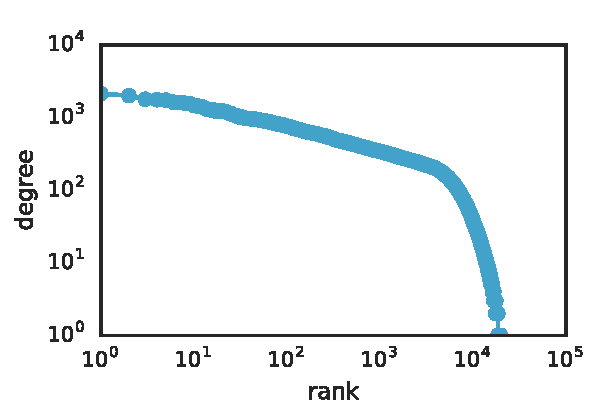
\includegraphics[width=0.6\textwidth]{./tex/chapter3/figures/170406_degree_rank_plot--GeneNet_1e+06_edges--title_deleted_inkscape.pdf}
    \begin{singlespace}
    % /Users/janet/Documents/Lidstrom Lab Work/meta4_bins_data_and_files/170406_GeneNet_on_the_largest_ledoit_Wolf_friendly_file--large_instance/170406_degree_rank_plot--GeneNet_1e+06_edges.svg
    \caption[Degree rank of plot for nodes in GeneNet derived partial correlation network]{
    	Degree rank of plot for nodes in GeneNet derived partial correlation network.
	The most connected nodes are shown on the left, and are each connected to more than 1,000 other genes.
	The least connected nodes have less than 10 connections.
        }
    \label{fig:degree_rank}
    \end{singlespace}
\end{figure}

Initial measures of the validity of the partial correlation matrix focused on the distribution of partial correlations for different sets of genes.
For example, the partial correlations of genes on the same contig are expected to be higher than partial correlations of genes on different contigs.
This turned out to be true (Figure \ref{fig:pcor_same_and_cross_contigs}).

\begin{figure}[H]
\centering
    % /Users/janet/Documents/Lidstrom Lab Work/meta4_bins_data_and_files/170412_explore_specific_network_as_done_previously/170412_explore_cutoff_0.01/same-contig_and_cross-contig_pcor_distributions.pdf
    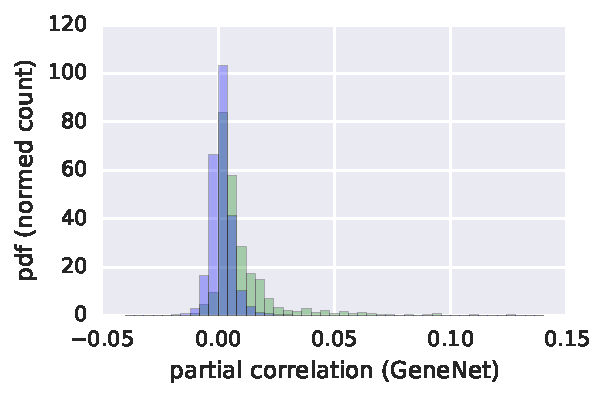
\includegraphics[width=0.6\textwidth]{./tex/chapter3/figures/same-contig_and_cross-contig_pcor_distributions.pdf}
    \begin{singlespace}
    % OLD: /Users/janet/Documents/Lidstrom Lab Work/meta4_bins_data_and_files/170406_GeneNet_on_the_largest_ledoit_Wolf_friendly_file--large_instance/170407_same-contig_and_cross-contig_pcor_distributions.pdf
    \caption[Distribution of partial correlations: same-contig versus across-contig gene pairs]{
    	Distribution of partial correlations: same-contig versus across-contig gene pairs, with each distribution normalized to have unit area.
	    Cross-contig gene pairs (blue bars, 997,276 edges) have lower partial correlations than pairs of genes found on the same contig (green bars, 2,724 edges).
        }
    \label{fig:pcor_same_and_cross_contigs}
    \end{singlespace}
\end{figure}

Similarly, higher partial correlations are expected between subunits of the same protein, or enzymes that are under the same regulation.
This hypothesis was tested by looking at the distribution of partial correlations between subunits of particulate methane monooxygenase \textit{pmo}.
All edges connecting pairs of \textit{pmo} genes were gathered and split into to sets: edges corresponding to the same \textit{pmo} cluster (sequential gene annotations on the same contig), and edges corresponding to two \textit{pmo} genes that are on different contigs or are not sequential.
The distributions (Figure \ref{fig:pmo_pcors}) confirm that subunits of the same operon have higher partial correlation values, adding validity to the GeneNet model.
The same is true for methanol dehydrogenase (\textit{mdh}) subunit pairs (Figure \ref{fig:mdh_pcors}) and hexulose-6-phosphate synthase:hexulose-6-phosphate isomerase gene pairs (Figure \ref{fig:hps_hpi_pcors}).

\begin{figure}[H]
\centering
    % /Users/janet/Documents/Lidstrom Lab Work/meta4_bins_data_and_files/170412_explore_specific_network_as_done_previously/170412_explore_cutoff_0.01/pmo_subunit_pairs_have_higher_pcor--GeneNet--1e+06_edges--horizontal.pdf
    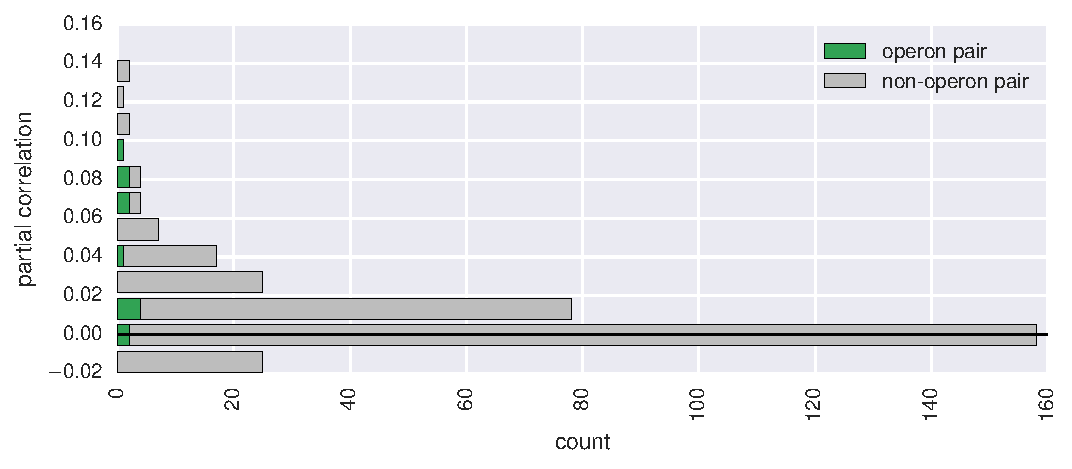
\includegraphics[width=1.0\textwidth]{./tex/chapter3/figures/pmo_subunit_pairs_have_higher_pcor--GeneNet--1e+06_edges--horizontal.pdf}
    \begin{singlespace}
    \caption[Partial correlation values for \textit{pmo}:\textit{pmo} subunit pairs]{
    	Partial correlation values for \textit{pmo}:\textit{pmo} subunit pairs in the GeneNet network.
	Green bars represent pairs that appear to be on the same operon, and gray bars represent all other pairs.
        }
    \label{fig:pmo_pcors}
    \end{singlespace}
\end{figure}

\begin{figure}[H]
\centering
    % /Users/janet/Documents/Lidstrom Lab Work/meta4_bins_data_and_files/170412_explore_specific_network_as_done_previously/170412_explore_cutoff_0.01/mdh-mdh_sequential_pairs--GeneNet--1e+06_genes--horizontal.pdf
    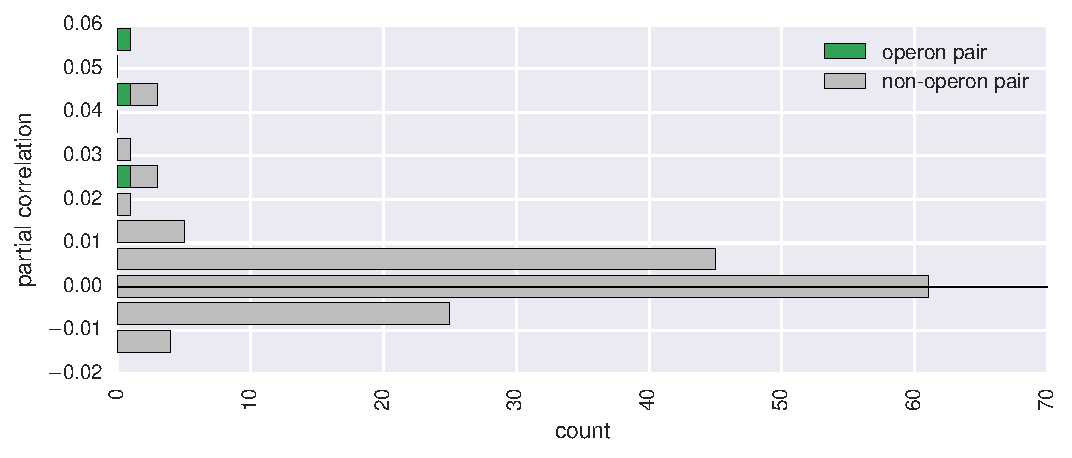
\includegraphics[width=1.0\textwidth]{./tex/chapter3/figures/mdh-mdh_sequential_pairs--GeneNet--1e+06_genes--horizontal.pdf}
    \begin{singlespace}
    \caption[Partial correlation values for \textit{mdh} subunit pairs]{
    	Partial correlation values for \textit{mdh} subunit pairs in the GeneNet network.
	    Green bars represent pairs that are sequential on a contig, and gray bars represent all other pairs.
        }
        \label{fig:mdh_pcors}
    \end{singlespace}
\end{figure}



\subsubsection{Future Directions for GeneNet Analysis}

This chapter identified great potential to use GeneNet for estimation of between-gene partial correlation values.
%There are many next steps for this early stage project.
%First, switching to measuring gene abundance in TPM could be considered, as a means to control for gene length.
%The current iteration used percent of reads in the \texttt{.fastq}, which shed light into how rare the included genes were in these samples, but give smaller %weights to  as the measure of expression for each gene.
%Switching to TPM (Transcripts Per Kilobase Million) could be used instead,
The next step is to mine these graphs for interesting biology.
Community structure can be detected by searching for groups of nodes that are highly connected to each other, but have fewer connections to nodes outside the group \cite{girvan2002}.
Layering in taxonomic labels for nodes will allow the ability to look at partial correlation values between species.

%It should also be possible to detect community structure using social network analysis algorithms.
%A variety are available, though algorithms that can account for edge weights can take advantage of the estimates of partial correlations.


%--------------------------- CCA RESULTS -------------------------------
\subsection{CCA}

CCA was run to see if subsets of genes expressed by methanotrophs have expression that is correlated with subsets of non-methanotrophic methylotroph genes.
The regularization path leading to the optimal objective function had penalties for both vectors equal to 0.026, indicating high regularization.
The vectors it selected for the methanotrophy and methylotrophy genes each included 5 genes, but a correlation of only 0.656.
The genes predicted did not point toward meaningful biology, either (Tables \ref{table:CCA_methanotroph}, \ref{table:CCA_methylotroph}).
This promising technique did not overcome the noise in these RNA-seq data.
Looking back to Figure \ref{fig:isolate_RNAseq}, these null results are likely due to low input data quality.
This method should be revisited when higher-confidence tabulated RNA-seq data becomes available, or used to target other questions.

\begin{table}[H]
\centering
\begin{singlespace}
\caption[Canonical correlation analysis: top features]{Canonical correlation analysis: top methanotroph features.}
\begin{tabular}{l | c | c}
 %\toprule
          gene number & gene name & coefficient  \\
\midrule
	1 & PEP-CTERM protein-sorting domain-containing  protein & 0.977  \\
	2 & heavy metal efflux pump, CzcA family &  0.053  \\
	3 & methionyl-tRNA synthetase &  0.028 \\
	4 & type I restriction enzyme M protein &  0.203 \\
	5 & zinc and cadmium transporter &  0.017 \\
%\bottomrule
\end{tabular}
\label{table:CCA_methanotroph}
\end{singlespace}
\end{table}

\begin{table}[H]
\centering
\begin{singlespace}
\caption[Canonical correlation analysis: top features]{Canonical correlation analysis: top methylotroph features.}
\begin{tabular}{l | c | c}
 %\toprule
          gene number & gene name & coefficient  \\
\midrule
	1 & 3-oxoacyl-[acyl-carrier protein] reductase & 0.214 \\
	2 & GMP synthase (glutamine-hydrolysing) & 0.735 \\
	3 & chaperonin GroEL & 0.544 \\
	4 & citrate synthase & 0.014 \\
	5 & phosphoglucosamine mutase & 0.341 \\
%\bottomrule
\end{tabular}
\label{table:CCA_methylotroph}
\end{singlespace}
\end{table}

% ==========================
% ===== CONCLUSIONS ========
% ==========================
\section{Conclusions}

This chapter described guidelines for applying statistical learning to metatranscriptomics datasets.
It warns against the common practice of centering features in data preprocessing.
Opportunities to use CCA and partial correlation graphs were highlighted.
Given the small $N$ and large $d$ characteristic of metatranscriptomics data, these models are recommended for hypothesis generation rather than predictive modeling.

Two promising software tools were demonstrated for explorations of partial correlation graphs: NetworkX and Neo4j.
NetworkX is powerful and easy to use for Python programmers.  It also has a lot of algorithms built in.
Neo4j has a more user friendly query language, but external packages are usually used when exploration algorithms are needed.

Applications of these techniques will be stronger after refining the tabulated RNA-seq data as is described in Chapter \ref{chapter:B}.

